\section{Proposed Methodology}
The basic focus of the current research is to extract feature requests and bug reports for popular
software systems and applications, as the discussions or user stories are readily available for
them. The classification is performed on the basis of applications, and not the specific
functionalities of these applications categories. However, there is not much benefit of it to the new
developers or developers of less popular systems. Since the functionalities in newer or less popular systems are more or less similar to the popular
applications, there could be a possibility that the information contained in the user stories of
popular applications can be made to use for newer systems. The proposed methodology
basically focusses on suggesting feature requests and bug reports on the basis of individual
functionalities of a software system and software category. Whenever a new developer wants to create a new
application, he selects the category for building his application. If devolper wants to see the new feature for his exisiting application he will specify the application.\\

	The database is populated based on the feedback from the classification and summarization
block. The purpose of the classification and the summarization block is to take input from the
existing social media and online platforms like Twitter, Facebook, App stores and LinkedIn etc.
So far only single study \cite{Nayebi} exist that takes data from two sources i.e. Twitter and app store.
Otherwise, the data from these sources were dealt separately. Different steps to be
performed are shown in Figure 1.

\begin{figure}
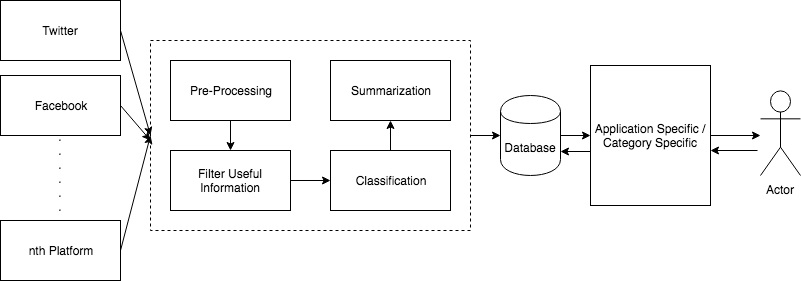
\includegraphics[width=\linewidth]{fig.png}
\caption{Block diagram of proposed methodology.}
\end{figure}

\textbf{Step 1 - Data Preprocessing: } The input data will be prepared for classification after preprocessing. This step will probably include tokenization, removal of stop words, stemming, etc. This step majorly depends on the chosen dataset combination, as different social media platforms have their limitations accordingly.\\

\textbf{Step 2 –  Filter useful information: } This step will gather and filter the selected App or category description data. Each application has a description on app stores and on their Twitter or Facebook page. This description will be helpful to determine the main feature of an application as relevant information. Also, some behavior feature will be learned.  For example how much is the company responsive and replies to the customer.This description data will be filtered upon the user selection. It can also be used in next step as metadata.\\

\textbf{Step 3 –  Classification: } Not all user discussions will be useful for feature requests or bug reports extraction. Therefore, it is necessary to filter out useful information from the other. The semi-supervised algorithm will learn a classifier. That will classify the data into a feature request, bug reports, and other categories.\\

\textbf{Step 4 – Summarization: } Multiple discussions could be related to the same feature or bug.
Since the datasets extracted from the sources is so massive, going through the complete datasets
would be humanly impossible. The information needs to be summarized so that the similar type
of information can be seen together. In this ranking process will consider features from the different sources such as likes, share, user behavior, sentiment analysis etc. As our dataset will be multi sourced, different features and their impact will be researched on each dataset for future selection.As the last step, all information will be clustered using topic modeling algorithm. This will
give developers and practitioner an idea of which feature requests or bug reports are more emphasized and frequently discussed as compared to the rest.\\

\subsection{User Interaction with the system:}
\begin{itemize}
\item{\textbf{Use Case 1:\\}}
 \underline {Name:} Getting requirements for building a new application\\
 \underline{Brief Description:} Actor wants to get user requirements for building a new application in a specified category e.g. sports, entertainment etc.\\
 \underline{Actors: } Devolpers, Requirement Analyst.\\
 \underline{Basic Flow:}
\begin {itemize}
\item{Actor will select the option for building a new application.}
\item{Actor will choose the category in which he wants to builds a new application}
\item{System will collect the online data related to the specified category.}
\item{System will apply data preprocessing on the collected data.}
\item{System will classify data as user requirement, bug repot and other.}
\item{System will provide a list of most influential and top ranked user requirements and bug reports in form of extractive summary.\\}
\end{itemize}
\item{\textbf{Use Case 2:\\}}

 \underline{Name:} Getting updated requirements for existing application\\
 \underline{Brief Description:} Actor wants to get user requirements for his existing application such as Facebook, YouTube etc.\\
 \underline{Actors: } Devolpers, Requirement Analyst.\\
 \underline{Basic Flow:}
\begin {itemize}
\item{Actor will select the option for the existing application.}
\item{Actor will choose his application from the list.}
\item{System will collect the online data related to the specific application. }
\item{System will apply data preprocessing on the collected data.}
\item{System will classify data as user requirement, bug repot and other.}
\item{System will provide a list of most influential and top ranked user requirements and bug reports in form of extractive summary.\\}
\end{itemize}

\item\textbf{ {Use Case 3:\\}}

 \underline {Name:} Getting updated requirements for existing application\\
 \underline{Brief Description:} Actor wants to get user requirements for his existing application such as Facebook, YouTube etc.\\
 \underline{Actors: } Devolpers, Requirement Analyst.\\
 \underline{Basic Flow:}
\begin {itemize}
\item{Actor will select the option comparison from the existing application}
\item{Actor will choose his application from the list.}
\item{Actor will choose applications for the comparison from the list.}
\item{System will collect relevant online data for the list defined by the user.}
\item{System will apply data preprocessing on the collected data.}
\item{System will classify data as user requirement, bug repot and other.}
\item{System will provide a list of most influential and top ranked user requirements and bug reports in form of extractive summary.}
\end{itemize}

\end{itemize}

\begin{comment}
\begin{itemize}

\item{As a first step user will choose either he wants to build a new version of an existing application or a new application. Also, the user will determine that he wants to analyze specific application such as Facebook, chrome etc. 
or specific application category such as books, photo and video, news etc.}
\item{In the second step, some behavioral and main features of the application will be learned from the provided description on applications pages and app stores.}
\item{In the next step, data will be gathered based on the first step for preprocessing. This step output the clean data for further steps.}
\item{After preprocessing, data will be classified into categories based on user choice in the first step.}
\item{In the last step, most influential and top-ranked requests (reviews, Tweets etc) will be provided as a user requirement or main feature according to the user selected choice.}

\end{itemize}
\end{comment}

	The main aim of the proposed methodology is to assist developers who want to develop a new
system or developers of a system with less number of users. With this technique, such
developers will be able to get the advantage of the user reported features requests and bug reports
from popular applications. Further, the information will be summarized on the basis of specific
functionalities. So, if a developer wants to include two functionalities that exist in WhatsApp,
and two functionalities that exist in Snapchat, he can easily see what are the feature requests
and bug reports individually for all of these functionalities. This will hopefully result in better
developed applications as required by users, quicker bug fixes even before the final release, and
better testing of the applications before and after release.